\Chapter{Tesztelés}

A fejezet célja hogy bemutassa és összehasonlítsa a teszteket, illetve az elért eredményeket. Mivel a benchmark programok használati módban eltérnek egymástól, megfigyelhető hogy egyes benchmark programnál, jelentősebb a kernel változók módosításainak hatásai.
Ezeket diagrammok és ábrák formájában próbálom összesíteni.
A benchmark tesztelési környeznek egy hagyományos asztali számítógépet használtam fel, amelynek hardveres és szoftveres specifikációi a következők.

\begin{lstlisting}
       _,met$$$$$gg.         davida@debian-pc 
    ,g$$$$$$$$$$$$$$$P.      ---------------- 
  ,g$$P"     """Y$$.".       OS: Debian GNU/Linux 10 x86_64 
 ,$$P'              `$$$.    Host: H81-D3 
',$$P       ,ggs.     `$$b:  Kernel: 5.8.5 
`d$$'     ,$P"'   .    $$$   Uptime: 2 hours, 25 mins 
 $$P      d$'     ,    $$P   Packages: 1669 (dpkg) 
 $$:      $$.   -    ,d$$'   Shell: bash 5.0.3 
 $$;      Y$b._   _,d$P'     Resolution: 1920x1080 
 Y$$.    `.`"Y$$$$P"'        WM: i3 
 `$$b      "-.__             Theme: Adwaita [GTK3] 
  `Y$$                       Icons: Adwaita [GTK3] 
   `Y$$.                     Terminal: urxvt 
     `$$b.                   CPU: Intel i5-4440 (4) 3.300GHz 
       `Y$$b.                GPU: AMD Radeon R7 265 1024SP 
          `"Y$b._            GPU: Intel HD Graphics 
              `"""           Memory: 1358MiB / 7844MiB
\end{lstlisting}
A neofetch program választottam erre a feladatra. Úgy gondoltam, hogy ez kellőképpen összegzi az szükséges adatokat. A Neofetch program, egy CLI-s rendszer információkat megjelenítő eszköz amelyet BASH-ben írtak [].


\Section{Benchmark tesztek elemzése}

Az openbenchmarking.org oldalon több mint 600 benchmark tesztprogram elérhető, amelyek különböző kategóriába lettek sorolva. A teszteléshez minden kategóriából választottam programokat, így szerettem volna szimulálni a különböző felhasználási módokat. Figyelembe kellett vegyem benchmark választásnál azt is a hogy, a programok viszonylag gyorsan végezzenek, mivel sok féle kombinációval kellett végrehajtanom ugyanazokat a teszteket. 

\SubSection{CPU intezív tesztek}

Az első felhasználási mód, a CPU-t terhelő benchmarkok kategóriája, ehhez két tesztet is választottam, névszerint a sampleprogramot illetve az ebizzyt.
Minden teszthez készítettem néhány diagrammot, amin megfigyelhető hogy, a különböző változók módosításával milyen eredmények születtek.

\begin{figure}[h!]
\centering
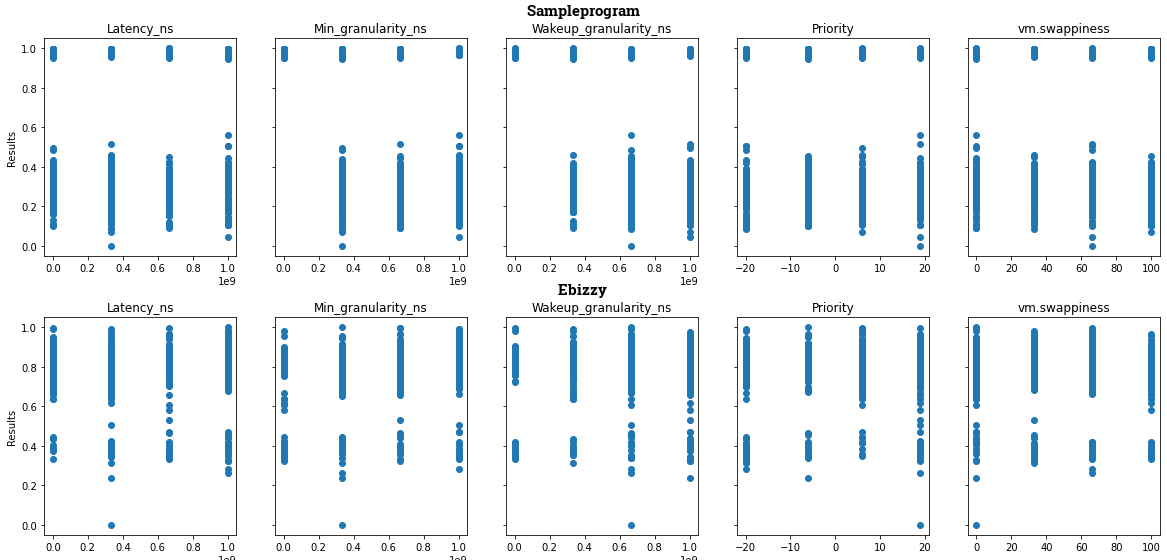
\includegraphics[scale=0.35]{images/cpuBenchmarkValues.png}
\caption{CPU benchmark eredményekhez tartozó kernel változók és prioritás értékek}
\label{fig:CpuParameters}
\end{figure}

Mint ahogy látjuk itt, a két benchmark teszteredményeit hasonlónak mondhatjuk. Mindkettőnél látható egy "hézag", ami elválasztja a jobb és a rossz eredményeket. Az eredmények romlása akkor jelentkezik amikor a sched\_wakeup\_granularity\_ns változóhoz nagyobb értékét állítunk mint a sched\_latency\_ns fele. Ekkor sajnos a kis időciklusú taszkok nem lesznek képesek versenyezni a többi folyamattal amikor a processzort éppen nagy terhelés alatt áll.
Az eredmények nagyrésze a legjobb kategóriába került, ez a sampleprogramnál 53\%, amíg az ebizzynél pedig 58\%. Ebből következtethetünk arra hogy a CPU intenzív felhasználási módhoz a legtöbb beállítás a kernel változókon, elfogadható teljesítményt eredményezett.

\SubSection{Rendszert terhelő benchmark}
Ebben a kategóriában nem processzor kimerítés hanemm, inkább a nagy rendszerhívás szám jellemzőbb.
A született eredmények nagyrésze a legjobb kategóriába került. Így azt mondhatom hogy, a intenzív rendszerterhelés felhasználási módhoz a legtöbb beállítás amit végeztem a kernel változókon, megfelelő teljesítményt eredményez. Minél több eredmény kerül a legjobb kategóriába, az ML program annál könnyebben fog tudni "jobb" értéket javasolni az adott felhasználási módhoz.


\SubSection{Videókártyát és memóriát terhelő benchmarkok}
A grafikus és memória benchmarkok, felhasználási módban és terhelésben is eltérnek egymástól, viszont mégis van bennük egy közös.
A grafikus benchmarkhoz készített ábrán(ami a változó értékeket jeleníti meg és az azokkal elért eredményeket), látható hogy itt is jelen van a cpu tesztnél már megfigyelt "hézag", a jobb illetve rosszabb értékek között, ami viszont a memória benchmarknál nem jelentkezik.

\begin{figure}[h!]
\centering
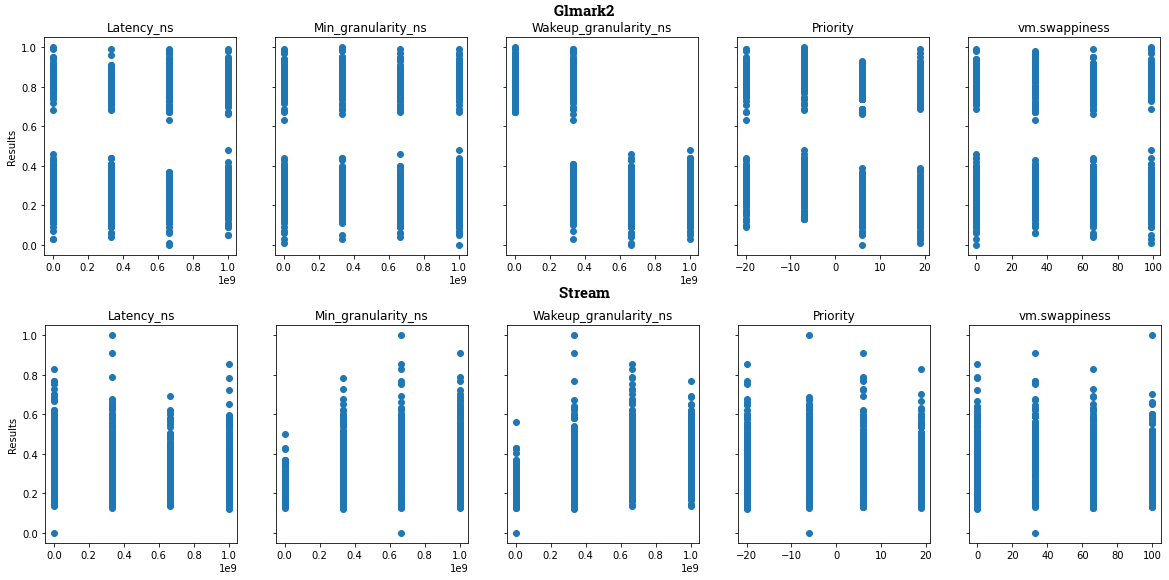
\includegraphics[scale=0.35]{images/graphicsAndMemoryBenchmarkValue.png}
\caption{Grafikus és memória benchmark eredményekhez tartozó kernel változók és prioritás értékek}
\label{fig:GraphicsAndMemoryParameters}
\end{figure}

A memória és grafikus benchmark közös tulajdonsága, az eredmény értékek eloszlása. Mindkét benchmarknál elmondható hogy az eredmények legnagyobb része, a legrosszabb kategóriába került.
Ezt a következő torta diagrammokról le is olvashatjuk.

\begin{figure}[h!]
\centering
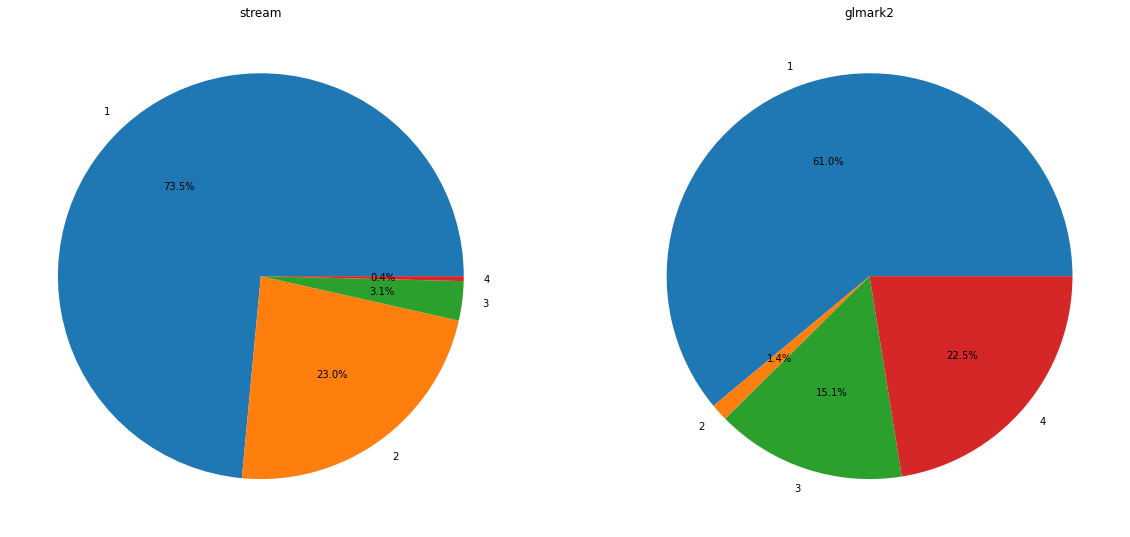
\includegraphics[scale=0.3]{images/graphicsAndMemoryBenchmarkChart.png}
\caption{Grafikus és memória benchmarkokból származó értékek}
\label{fig:GraphicsAndMemoryChart}
\end{figure}

Így a 3-as, 4-es kategóriába tartozó eredmények ritkának mondhatók. Amennyiben megfigyeljük az adathalmazt hogy mi is váltotta ki ezeket, észrevehetjük hogy a memória benchmarknál  minden "jobb" eredmény eléréséhez szükség volt a szerver szintű terhelési mód beállítására.
A grafikus benchmarknál sajnos, nem találtam szabad szemmel látható összefüggéseket, így a legjobb beállítási értékek megválasztását az ML programra bíztam.

\SubSection{Háttértárat terhelő benchmark}
A háttértárakat terhelő benchmark kategória tipikusan az, ahol a processzek az életük nagyrészét I/O-ra történő várakozzással töltik.
Az itt kapott eredmények nagy része 1-es illetve 2-es kategóriába került, ezeket vehetjük úgymond átlagos értékeknek. Mivel a legtöbb érték a legrosszabb eredmények halmazaiba kerültek, feltételezhetjük hogy néhány beállítás elősegítette a jobb értékek kialakulását. 
Fontos kiemelnem hogy, a módosított változó értékek nem függetlenek egymástól, emiatt nem feltételezhetjük azt hogyha, a legjobb értékekeket elért változókat kiválasztjuk, megkapjuk a tökéletes beállítást az ütemező hangolására.

\begin{figure}[h!]
\centering
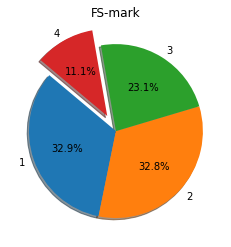
\includegraphics[scale=0.6]{images/diskBenchmarkValue.png}
\caption{Háttértárakat terhelő benchmarkból származó értékek.}
\label{fig:diskChart}
\end{figure}


